% % !TeX root = tcolorbox.tex
% % include file of tcolorbox.tex (manual of the LaTeX package tcolorbox)
% \clearpage
\section{Libraries
  \mylib{listings},
  \mylib{listingsutf8}, and
  \mylib{minted}}\label{sec:listings}%
\tcbset{external/prefix=external/listings_}%


% \include*{listings/加载库}
% \include*{listings/加载listings}
% \subsection{Common Macros of the Libraries\\库的常用宏}
% \include*{listings/库的常用宏_tcblisting}
% \include*{listings/库的常用宏_写入文件}\include*{listings/库的常用宏_读取文件} % tcolorbox.listing
% \include*{listings/库的常用宏_newtcblisting}
% \include*{listings/库的常用宏_新建读取文件}
% \include*{listings/listings库的选项键}\subsection{Option Keys of the \mylib{listingsutf8} Library\\listingsutf8库的选项键}

\begin{marker}
The \mylib{listingsutf8} library is not needed (and troublesome) when using Xe\LaTeX\ or Lua\LaTeX.
Therefore, loading this library is automatically replaced by loading
\mylib{listings} only, if pdf\LaTeX\ is \emph{not} used.

当使用 Xe\LaTeX\ 或 Lua\LaTeX 时,不需要(而且可能会有问题)加载 \mylib{listingsutf8} 库。 因此,如果不使用 pdf\LaTeX,加载此库会自动替换为仅加载 \mylib{listings}。
\end{marker}

The \mylib{listingsutf8} library is an extension of the
\mylib{listings} library, so
all options from \Vref{sec:speclistingkeys} are applicable.

\mylib{listingsutf8} 库是 \mylib{listings} 库的扩展,因此 \Vref{sec:speclistingkeys} 中的所有选项都适用。
\begin{docTcbKey}{listing utf8}{=\meta{one-byte-encoding}}{style, no default, initially |latin1|}
Abbreviation for using \refKeyLe{/tcb/listing inputencoding}
together with UTF-8 support from the package |listingsutf8| .
This option is available only for the library variant \mylib{listingsutf8}.
The \meta{one-byte-encoding} is one of
the applicable encodings from , e.\,g.\ |latin1|
which is the default.\par

% 使用\refKeyLe{/tcb/listing inputencoding}的缩写,结合来自包|listingsutf8|的UTF-8支持。此选项仅适用于库变体\mylib{listingsutf8}。\meta{one-byte-encoding}是来自的适用编码之一,例如|latin1|是默认值。

使用\refKeyLe{/tcb/listing inputencoding}和来自|listingsutf8|包的UTF-8支持的缩写。此选项仅适用于库变体\mylib{listingsutf8}。 \meta{one-byte-encoding} 是可适用的编码之一,例如|latin1|是默认值。

Be aware that this means restriction to this specific \meta{one-byte-encoding}:
e.\,g.\ |latin1| comprises umlauts and other accented characters, but not
the Euro sign. If you want to use the |listings| package \emph{and} \flqq real\frqq\
UTF-8 source code, then do \emph{not} use \mylib{listingsutf8} but \mylib{listings}
with
\refKeyLe{/tcb/listing inputencoding}|=utf8|
\emph{and} with specific manual hacks for specific UTF-8-encoded characters.

% 请注意,这意味着限制在特定的\meta{one-byte-encoding}上:例如|latin1|包括umlauts和其他重音字符,但不包括欧元符号。如果您想同时使用|listings|包和“真正的”UTF-8源代码,则不要使用\mylib{listingsutf8},而是使用\mylib{listings},并使用\refKeyLe{/tcb/listing inputencoding}|=utf8|以及针对特定UTF-8编码字符的手动修补。

请注意,这意味着限制于特定的 \meta{单字节编码}: 例如,|latin1| 包含变音符和其他有重音符号的字符,但不包括欧元符号。如果您想使用 |listings| 宏包并使用“真正”的 UTF-8 源代码,则不要使用 \mylib{listingsutf8},而应该使用带有 \refKeyLe{/tcb/listing inputencoding}|=utf8| 的 \mylib{listings},并且使用特定的手动修改来处理特定的 UTF-8 编码字符。
\end{docTcbKey}

See further options in \Vref{sec:commonlistingkeys}.

请参阅 \Vref{sec:commonlistingkeys} 中的其他选项。
%\include*{listings/minted库的选项键}
% For the \meta{options} in \refEnv{tcblisting} respectively \refCom{tcbinputlisting}
the following |pgf| keys can be applied. The key tree path |/tcb/| is not to
be used inside these macros.

对于\refEnv{tcblisting}或\refCom{tcbinputlisting}中的\meta{options},可以应用以下|pgf|键。不应在这些宏中使用键树路径|/tcb/|。
\begin{docTcbKey}{listing engine}{=\meta{engine}}{no default}
Sets the \meta{engine} which typesets the listings. Feasible values are

设置排版代码的\meta{engine}。可行的值为: %\begin{itemize} \item 如果加载了库\mylib{listings}或\mylib{listingsutf8},则为\docValue{listings}。 \item 如果加载了库\mylib{minted},则为\docValue{minted}。 \end{itemize}
\begin{itemize}
\item\docValue{listings}, if library \mylib{listings} or
\mylib{listingsutf8} is loaded.
\item\docValue{minted}, if library \mylib{minted} is loaded.
\end{itemize}
\end{docTcbKey}

\begin{docTcbKey}{listing file}{=\meta{file name}}{no default, initially \cs{jobname.listing}}
Sets the \meta{file name} of the file which is used to save listings.

设置用于保存代码清单的文件的\meta{文件名}。
\end{docTcbKey}


\begin{docTcbKey}{listing and text}{}{no value, initially set}
Typesets the environment content as listing in the upper part and
as compiled text in the lower part.

将环境内容分别作为源码清单显示在上部和编译后的文本显示在下部。
\begin{dispExample}
\begin{tcblisting}{colback=red!5!white,colframe=red!75!black,listing and text}
This is a \LaTeX\ example.
\end{tcblisting}
\end{dispExample}
\end{docTcbKey}


\begin{docTcbKey}{text and listing}{}{no value}
Typesets the environment content as compiled text in the upper part and
as listing in the lower part.

将环境内容分别作为源码清单显示在上部和编译后的文本显示在下部。
\begin{dispExample}
\begin{tcblisting}{colback=red!5!white,colframe=red!75!black,text and listing}
This is a \LaTeX\ example.
\end{tcblisting}
\end{dispExample}
\end{docTcbKey}


\begin{docTcbKey}{listing only}{}{no value}
Typesets the environment content as listing.

将环境内容排版为清单形式。
\begin{dispExample}
\begin{tcblisting}{colback=red!5!white,colframe=red!75!black,listing only}
This is a \LaTeX\ example.
\end{tcblisting}
\end{dispExample}
\end{docTcbKey}


%%\clearpage
\begin{docTcbKey}{text only}{}{no value}
Typesets the environment content as compiled text.

将环境内容排版为已编译的文本。
\begin{dispExample}
\begin{tcblisting}{colback=red!5!white,colframe=red!75!black,text only}
This is a \LaTeX\ example.
\end{tcblisting}
\end{dispExample}
\end{docTcbKey}



\begin{docTcbKey}{comment}{=\meta{text}}{no default, initially empty}
Records a comment with \meta{text} as content. The comment is displayed
e.\,g.\ in conjunction with \refKey{/tcb/listing and comment}
and \refKey{/tcb/comment and listing}.

记录一个以 \meta{text} 为内容的注释。该注释通常与 \refKey{/tcb/listing and comment} 和 \refKey{/tcb/comment and listing} 一起显示。
\begin{dispExample}
\begin{tcblisting}{comment={This comment is really only a comment},
colback=red!5!white,colframe=red!75!black}
This is a \textbf{tcolorbox}.
\end{tcblisting}
\end{dispExample}
\end{docTcbKey}


\begin{docTcbKey}[][doc new=2014-11-17]{comment only}{}{no value}
Typesets the environment content with the comment text.

使用注释文本对环境内容进行排版。
\begin{dispExample}
\begin{tcblisting}{comment only,
comment={This is a comment.},
colback=red!5!white,colframe=red!75!black}
This is a \textbf{tcolorbox}.
\end{tcblisting}
\end{dispExample}
\end{docTcbKey}



\begin{docTcbKey}{image comment}{=\marg{options}\marg{filename}}{style, no default, initially unset}
Uses an image denoted by \meta{filename} as \textit{comment} for the listing.
The image is included by the standard |\includegraphics| macro with
given \meta{options}.

使用由\meta{filename}表示的图像作为源码清单的\textit{注释}。 该图像通过标准的|\includegraphics|宏和给定的\meta{options}被包含进来。
\begin{dispExample}
\begin{tcblisting}{colback=red!5!white,colframe=red!75!black,listing side comment,
image comment={width=2.5cm}{example-image-a.pdf},center lower}
This is a \LaTeX\ example.
\end{tcblisting}
\end{dispExample}
\end{docTcbKey}


%%\clearpage
\begin{docTcbKey}[][doc new=2014-11-14]{tcbimage comment}{=\meta{filename}}{style, no default, initially unset}
Uses an image denoted by \meta{filename} as \textit{comment} for the listing.
The image is included by the \refCom{tcbincludegraphics} macro.
The inclusion can be customized by \refKey{/tcb/comment style}.

使用由\meta{filename}指定的图像作为源码清单的\textit{注释}。 该图像由\refCom{tcbincludegraphics}宏包含。 包含可以通过\refKey{/tcb/comment style}进行自定义。
\begin{marker}
The library \mylib{skins} is needed to apply this option.

需要使用库\mylib{skins}来应用此选项。
\end{marker}
\medskip
\begin{dispExample}
% \tcbuselibrary{skins}
\begin{tcblisting}{colback=red!5!white,colframe=red!75!black,listing side comment,
righthand width=3cm,lower separated=false,
tcbimage comment={example-image-a.pdf},
comment style={size=fbox,colframe=blue,colback=blue!50,sharp corners,
drop fuzzy shadow}}
This is a \LaTeX\ example.
\end{tcblisting}
\end{dispExample}
\end{docTcbKey}

%%\clearpage

\begin{docTcbKey}[][doc new=2014-11-14]{pdf comment}{\colOpt{=\meta{filename}}}{style, default listing file, initially unset}
Uses a PDF file denoted by \meta{filename} as \textit{comment} for the listing.
The image is included by \refCom{tcbincludepdf} inside a \refEnv{tcbraster}.
The inclusion can be customized by \refKey{/tcb/comment style}.

使用由\meta{filename}表示的PDF文件作为清单的\textit{注释}。 图像由\refCom{tcbincludepdf}包含在\refEnv{tcbraster}中。 可以通过\refKey{/tcb/comment style}自定义包含。
\begin{marker}
The libraries \mylib{skins} and \mylib{raster} are needed to apply this option.

应用此选项需要 \mylib{skins} 和 \mylib{raster} 库。
\end{marker}
\medskip
\begin{dispExample}
% \tcbuselibrary{skins,raster}
\begin{tcblisting}{colback=red!5!white,colframe=red!75!black,listing and comment,
righthand width=3cm,lower separated=false,middle=1mm,
pdf comment={tcolorbox-example.pdf},
comment style={raster columns=3,graphics pages={1,2,3},
colframe=blue,drop fuzzy shadow}}
This is a \LaTeX\ example.
\end{tcblisting}
\end{dispExample}
\end{docTcbKey}

%%\clearpage


\begin{docTcbKey}[][doc new=2014-11-14]{pdf extension}{=\meta{extension}}{no default, initially |pdf|}
Sets the PDF file name extension for \refKey{/tcb/pdf comment} to \meta{extension}.
Note that \meta{extension} always overwrites any actual extension given
inside \refKey{/tcb/pdf comment}.

将 \refKey{/tcb/pdf comment} 的 PDF 文件名扩展名设置为 \meta{extension}。 请注意,\meta{extension} 总是覆盖 \refKey{/tcb/pdf comment} 中给定的实际扩展名。
\end{docTcbKey}


\begin{docTcbKey}[][doc new=2014-11-14]{comment style}{=\meta{options}}{no default, initially empty}
Sets the \meta{options} for \refKey{/tcb/tcbimage comment} and \refKey{/tcb/pdf comment}.
These are |tcolorbox| options to customize the colored box drawn around the
image(s), also image options encapsulated by \refKey{/tcb/graphics options},
and \refEnv{tcbraster} options for \refKey{/tcb/pdf comment}.

设置\refKey{/tcb/tcbimage comment}和\refKey{/tcb/pdf comment}的\meta{options}。 这些都是用于自定义围绕图像绘制的彩色框的|tcolorbox|选项, 还包括由\refKey{/tcb/graphics options}封装的图像选项, 以及用于\refKey{/tcb/pdf comment}的\refEnv{tcbraster}选项。
\end{docTcbKey}


\begin{docTcbKey}{listing and comment}{}{no value}
Typesets the environment content as listing in the upper part and
a given comment in the lower part.

将环境内容排版为上部的源码清单形式,下部为给定的注释。
\begin{dispExample}
\begin{tcblisting}{colback=red!5!white,colframe=red!75!black,listing and comment,
comment={This is my comment. It may contain line breaks.\par
It can even use the environment content
\flqq\ignorespaces\tcbuselistingtext\unskip\frqq}}
This is a \LaTeX\ example.
\end{tcblisting}
\end{dispExample}
\end{docTcbKey}

\enlargethispage*{10mm}
\begin{docTcbKey}{comment and listing}{}{no value}
Typesets a given comment in the upper part and
the environment content as listing in the lower part.

将给定的注释排版在上部,将环境内容作为源码清单排列在下部。
\begin{dispExample}
\begin{tcblisting}{colback=red!5!white,colframe=red!75!black,comment and listing,
comment={This is my comment.}}
This is a \LaTeX\ example.
\end{tcblisting}
\end{dispExample}
\end{docTcbKey}


%%\clearpage
\begin{docTcbKey}{listing side text}{}{style, no value}
Typesets the environment content side by side as listing in the left (upper)
part and as compiled text in the right (lower) part.
This is a shortcut for setting \refKey{/tcb/listing and text} and \refKey{/tcb/sidebyside}.

将环境内容并排设置为左侧(上部)的清单和右侧(下部)已编译文本。 这是设置 \refKey{/tcb/listing and text} 和 \refKey{/tcb/sidebyside} 的快捷方式。
\begin{dispExample}
\begin{tcblisting}{colback=red!5!white,colframe=red!75!black,listing side text}
This is a \LaTeX\ example.
\end{tcblisting}
\end{dispExample}
\begin{marker}
Note that |sidebyside=false| has to be added, if the setting of
\refKey{/tcb/listing side text} is to be annihilated.

请注意,如果要取消\refKey{/tcb/listing side text}的设置,则必须添加|sidebyside=false|。
\end{marker}
\end{docTcbKey}


\begin{docTcbKey}{text side listing}{}{style, no value}
Typesets the environment content side by side as compiled text in the left (upper)
part and as listing in the right (lower) part.
This is a shortcut for setting \refKey{/tcb/text and listing} and \refKey{/tcb/sidebyside}.

将环境内容排列在左侧(上部)以编译文本的形式,右侧(下部)以清单的形式并排显示。 这是一种快捷方式,用于设置 \refKey{/tcb/text and listing} 和 \refKey{/tcb/sidebyside}。
\begin{dispExample}
\begin{tcblisting}{colback=red!5!white,colframe=red!75!black,text side listing}
This is a \LaTeX\ example.
\end{tcblisting}
\end{dispExample}
\end{docTcbKey}


\begin{docTcbKey}{listing outside text}{}{no value}
Typesets the environment content side by side as listing in a |tcolorbox|
and as compiled text outside the box in the right part of the page.
Nevertheless, the outside text is treated as \emph{lower} part of the
|tcolorbox| and can be formatted with all lower part options.
The space partitioning is done with the side by side options from
\Fullref{sec:sidebyside}.

在 |tcolorbox| 中,将环境内容并排列出来,作为清单,并将编译文本放在页面右侧的盒子外部。尽管如此,外部文本被视为 |tcolorbox| 的 \emph{下部分},可以使用所有下部分选项进行格式化。空间分区使用来自\Fullref{sec:sidebyside}的并排选项进行。
\begin{dispExample}
\begin{tcblisting}{colback=red!5!white,colframe=red!75!black,listing outside text}
This is a \LaTeX\ example.
\end{tcblisting}
\end{dispExample}
\end{docTcbKey}

%%\clearpage

\begin{docTcbKey}{text outside listing}{}{no value}
Typesets the environment content side by side as listing in a |tcolorbox|
and as compiled text outside the box in the left part of the page.
Nevertheless, the outside text is treated as \emph{lower} part of the
|tcolorbox| and can be formatted with all lower part options.
The space partitioning is done with the side by side options from
\Fullref{sec:sidebyside}.

将环境内容在|tcolorbox|中侧面列出,并将已编译的文本放在页面左侧的框外。尽管如此,外部文本被视为|tcolorbox|的\emph{下部},并且可以使用所有下部选项进行格式化。空间分区是使用\Fullref{sec:sidebyside}中的并排选项完成的。
\begin{dispExample}
\begin{tcblisting}{colback=red!5!white,colframe=red!75!black,text outside listing}
This is a \LaTeX\ example.
\end{tcblisting}
\end{dispExample}
\end{docTcbKey}



\begin{docTcbKey}{listing side comment}{}{style, no value}
Typesets the environment content side by side as listing in the left (upper)
part and a given comment in the right (lower) part.
This is a shortcut for setting \refKey{/tcb/listing and comment} and \refKey{/tcb/sidebyside}.

将环境内容排列在左侧(上部)的清单中,给定的注释排列在右侧(下部)。 这是设置\refKey{/tcb/listing and comment}和\refKey{/tcb/sidebyside}的快捷方式。
\begin{dispExample}
\begin{tcblisting}{colback=red!5!white,colframe=red!75!black,listing side comment,
righthand width=1.5cm,image comment={width=1.5cm}{example-image-a.pdf}}
This is a \LaTeX\ example.
\end{tcblisting}
\end{dispExample}
\end{docTcbKey}


\begin{docTcbKey}{comment side listing}{}{style, no value}
Typesets the environment content side by side with a given comment in the left (upper)
part and as listing in the right (lower) part.
This is a shortcut for setting \refKey{/tcb/comment and listing} and \refKey{/tcb/sidebyside}.

将环境内容与给定注释一起排列在左侧(上部),并将源码清单排列在右侧(下部)。 这是设置\refKey{/tcb/comment and listing}和\refKey{/tcb/sidebyside}的快捷方式。
\begin{dispExample}
\begin{tcblisting}{colback=red!5!white,colframe=red!75!black,comment side listing,
lefthand width=1.5cm,image comment={width=1.5cm}{example-image-a.pdf}}
This is a \LaTeX\ example.
\end{tcblisting}
\end{dispExample}
\end{docTcbKey}

%%\clearpage

\begin{docTcbKey}{listing outside comment}{}{no value}
Typesets the environment content side by side as listing in a |tcolorbox|
and a given comment outside the box in the right part of the page.
Nevertheless, the outside text is treated as \emph{lower} part of the
|tcolorbox| and can be formatted with all lower part options.
The space partitioning is done with the side by side options from
\Fullref{sec:sidebyside}.

将环境内容与给定评论并排作为源码清单在 |tcolorbox| 中排列,并在页面右侧的框外给出评论。然而,外部文本被视为 |tcolorbox| 的\emph{下部分},可以使用所有下部分选项进行格式化。空间划分是使用 \Fullref{sec:sidebyside} 中的并排选项完成的。
\begin{dispExample}
\begin{tcblisting}{colback=red!5!white,colframe=red!75!black,listing outside comment,
righthand width=1.5cm,image comment={width=1.5cm}{example-image-a.pdf}}
This is a \LaTeX\ example.
\end{tcblisting}
\end{dispExample}
\end{docTcbKey}


\begin{docTcbKey}{comment outside listing}{}{no value}
Typesets the environment content side by side as listing in a |tcolorbox|
and a given comment outside the box in the left part of the page.
Nevertheless, the outside text is treated as \emph{lower} part of the
|tcolorbox| and can be formatted with all lower part options.
The space partitioning is done with the side by side options from
\Fullref{sec:sidebyside}.

在 |tcolorbox| 中将环境内容并排设置为源码清单,并在页面左侧给出给定的注释。然而,外部文本被视为 |tcolorbox| 的 \emph{下部} 部分,并且可以使用所有下部选项进行格式化。空间划分是通过从 \Fullref{sec:sidebyside} 中的并排选项完成的。
\begin{dispExample}
\begin{tcblisting}{colback=red!5!white,colframe=red!75!black,comment outside listing,
lefthand width=1.5cm,image comment={width=1.5cm}{example-image-a.pdf}}
This is a \LaTeX\ example.
\end{tcblisting}
\end{dispExample}
\end{docTcbKey}



\begin{docTcbKey}{listing above text}{}{no value}
Typesets the environment content as listing in a |tcolorbox|
and as compiled text outside and below the box.
The outside text is treated as \emph{lower} part of the
|tcolorbox| and can be formatted with all lower part options.
The distance between box and text is controlled by \refKey{/tcb/middle}.

将环境内容排版为 |tcolorbox| 中的清单,并将已编译的文本放在盒子之外和下方。盒子外的文本被视为 |tcolorbox| 的 \emph{下部},可以使用所有下部选项进行格式化。盒子和文本之间的距离由 \refKey{/tcb/middle} 控制。
\begin{dispExample}
\begin{tcblisting}{colback=red!5!white,colframe=red!75!black,listing above text}
This is a \LaTeX\ example.
\end{tcblisting}
\end{dispExample}
\end{docTcbKey}


\begin{docTcbKey}[][doc new=2014-11-07]{listing above* text}{}{no value}
Widely equal to \refKey{/tcb/listing above text}, but the outside text is
not formatted with the lower part options.
Also, it is not put into a minipage and it may span several pages.
The distance between box and text is controlled by \refKey{/tcb/after}.

与\refKey{/tcb/listing above text}基本相同,但外部文本不使用底部选项格式化。此外,它不会放入一个小页中,可能跨越多个页面。盒子和文本之间的距离由\refKey{/tcb/after}控制。
\end{docTcbKey}

%%\clearpage

\begin{docTcbKey}{text above listing}{}{no value}
Typesets the environment content as listing in a |tcolorbox|
and as compiled text outside and above the box.
The outside text is treated as \emph{lower} part of the
|tcolorbox| and can be formatted with all lower part options.
The distance between box and text is controlled by \refKey{/tcb/middle}.

将环境内容排版为 |tcolorbox| 中的源码清单,并编译成文本在盒子外部和上方。外部文本被视为 |tcolorbox| 的 \emph{下部} 部分,并可以使用所有下部选项进行格式化。盒子和文本之间的距离由 \refKey{/tcb/middle} 控制。
\begin{dispExample}
\begin{tcblisting}{colback=red!5!white,colframe=red!75!black,text above listing}
This is a \LaTeX\ example.
\end{tcblisting}
\end{dispExample}
\end{docTcbKey}


\begin{docTcbKey}[][doc new=2014-11-07]{text above* listing}{}{no value}
Widely equal to \refKey{/tcb/text above listing}, but the outside text is
not formatted with the lower part options.
Also, it is not put into a minipage and it may span several pages.
The distance between box and text is controlled by \refKey{/tcb/before}.

与 \refKey{/tcb/text above listing} 相似,但是外部文本不使用下部选项进行格式化。此外,它不会被放入一个小页中,也可能跨越多个页面。盒子和文本之间的距离由 \refKey{/tcb/before} 控制。
\end{docTcbKey}



\begin{docTcbKey}{listing above comment}{}{no value}
Typesets the environment content as listing in a |tcolorbox|
and a given comment outside and below the box.
The outside text is treated as \emph{lower} part of the
|tcolorbox| and can be formatted with all lower part options.
The distance between box and comment is controlled by \refKey{/tcb/middle}.

将环境内容排版为源码清单形式,放置在一个 |tcolorbox| 中,并在盒子外部和下方给出注释。外部文本被视为 |tcolorbox| 的 \emph{下部} 部分,可以使用所有下部选项进行格式化。盒子和注释之间的距离由 \refKey{/tcb/middle} 控制。
\begin{dispExample}
\begin{tcblisting}{colback=red!5!white,colframe=red!75!black,listing above comment,
center lower,image comment={width=3cm}{example-image-a.pdf}}
This is a \LaTeX\ example.
\end{tcblisting}
\end{dispExample}
\end{docTcbKey}


\begin{docTcbKey}[][doc new=2014-11-07]{listing above* comment}{}{no value}
Widely equal to \refKey{/tcb/listing above comment}, but the outside comment is
not formatted with the lower part options.
Also, it is not put into a minipage and it may span several pages.
The distance between box and comment is controlled by \refKey{/tcb/after}.

与 \refKey{/tcb/listing above comment} 大致相同,但外部注释不使用底部选项格式化。此外,它不会放置在一个小页中,可能跨越多个页面。盒子与注释之间的距离由 \refKey{/tcb/after} 控制。
\end{docTcbKey}

%%%%\clearpage

\begin{docTcbKey}{comment above listing}{}{no value}
Typesets the environment content as listing in a |tcolorbox|
and a given comment outside and above the box.
The outside text is treated as \emph{lower} part of the
|tcolorbox| and can be formatted with all lower part options.
The distance between box and comment is controlled by \refKey{/tcb/middle}.

将环境内容设置为 |tcolorbox| 中的源码清单,并在框外和上方给出注释。外部文本被视为 |tcolorbox| 的 \emph{下部} 部分,并可以使用所有下部选项进行格式化。框和注释之间的距离由 \refKey{/tcb/middle} 控制。
\begin{dispExample}
\begin{tcblisting}{colback=red!5!white,colframe=red!75!black,comment above listing,
center lower,image comment={width=3cm}{example-image-a.pdf}}
This is a \LaTeX\ example.
\end{tcblisting}
\end{dispExample}
\end{docTcbKey}


\begin{docTcbKey}[][doc new=2014-11-07]{comment above* listing}{}{no value}
Widely equal to \refKey{/tcb/comment above listing}, but the outside comment is
not formatted with the lower part options.
Also, it is not put into a minipage and it may span several pages.
The distance between box and comment is controlled by \refKey{/tcb/before}.

与\refKey{/tcb/comment above listing}大致相同,但外部注释没有使用底部选项进行格式化。并且,它没有放置在一个小页面中,可能跨越多个页面。盒子和注释之间的距离由\refKey{/tcb/before}控制。
\end{docTcbKey}

% \include*{listings/处理和完整文档示例的选项键}
% % \clearpage


The following source code gives a guideline for the creation of \LaTeX\ tutorials.
In the next section, a framework for \LaTeX\ exercises is described.
All examples shall be numbered optionally.

以下源代码提供了创建 \LaTeX\ 教程的指南。 在下一节中,描述了 \LaTeX\ 练习的框架。 所有示例均可选择编号。

Firstly, some additional |tcb| keys are defined for the appearance.
For the examples, three environments |texexp|, |texexptitled|,
and |texexptitledspec| are defined with automatic numbering.

首先,为了外观方面定义了一些额外的 |tcb| 键。为了举例,定义了三个环境,即带自动编号的 |texexp|、|texexptitled| 和 |texexptitledspec|。
\begin{itemize}
\item |texexp| is used for untitled examples,
\\|texexp| 用于无标题的例子,
\item |texexptitled| is used for titled examples,
\\|texexptitled| 用于带标题的例子,
\item |texexptitledspec| is used for titled examples with special treatment.
\\|texexptitledspec| 用于带特殊处理的标题例子。
\end{itemize}

\inputpreamblelisting{D}

\begin{dispExample}
\begin{tcblisting}{texexp}
This is a \LaTeX\ example which displays the text as source code
and in compiled form.

这是一个展示文本源代码和编译后形式的 \LaTeX\ 示例。
\end{tcblisting}
\end{dispExample}


\begin{dispExample}
\begin{texexptitled}{First example with a title line}{firstExample}
Here, we use Example \ref{firstExample} with a title line.

在这里,我们使用带有标题行的示例\ref{firstExample}。
\end{texexptitled}
\end{dispExample}


\begin{dispExample}
\begin{texexp}{}
This is a \LaTeX\ example which displays the text as source code
and in compiled form.

这是一个 \LaTeX\ 的示例,它可以将文本显示为源代码和编译后的形式。
\end{texexp}
\end{dispExample}


\begin{dispExample}
\begin{texexp}{text and listing}
This is a \LaTeX\ example which displays the text as source code
and in compiled form.

这是一个 \LaTeX\ 的示例,它展示了文本的源代码和编译后的形式。
\end{texexp}
\end{dispExample}


\begin{dispExample}
\begin{texexp}{listing only}
This is a \LaTeX\ example which displays the text as source code only.

这是一个 \LaTeX\ 的例子,仅以源代码形式显示文本。
\end{texexp}
\end{dispExample}


\begin{dispExample}
\begin{texexp}{text only}
This is a \LaTeX\ example which displays the text in compiled form only.

这是一个 \LaTeX\ 示例,仅以编译后的形式展示文本。
\end{texexp}
\end{dispExample}


\begin{dispExample}
\begin{texexptitled}{An Example with a Heading}{heading1}
This is a \LaTeX\ example with a numbered heading line
which can be referred to.

这是一个带有编号标题行的 \LaTeX\ 示例,可以进行引用。
\end{texexptitled}
Here, we see Example \ref{heading1}.

在这里,我们看到示例\ref{heading1}。
\end{dispExample}


\begin{dispExample}
\begin{texexptitled}[listing only]{Another Example with a Heading}{heading2}
The keys can be used in combination. Here, an example with a heading line
and source code only is given.

这些键可以组合使用。下面是仅包含标题和源代码的示例。
\end{texexptitled}
Here, we see Example \ref{heading2}.

在这里,我们看到示例 \ref{heading2}。
\end{dispExample}


\begin{dispListing}
\begin{texexptitled}[float]{A floating Example with a Heading}{heading3}
This is another \LaTeX\ example with numbered heading line.
But now, the box is a floating object.

这是另一个带有编号标题行的 \LaTeX\ 示例。 但现在,这个框是一个浮动对象。
\end{texexptitled}
\end{dispListing}
\tcbusetemp

\begin{dispExample}
The floating box of the last example is seen as Example \ref{heading3}
on page \pageref{heading3}.

上一个例子中的浮动框在第\pageref{heading3}页被视为第\ref{heading3}个例子。
\end{dispExample}


\begin{dispExample}
\begin{texexptitledspec}{Special application}{texexpbox1}
\begin{lstlisting}[style=tcblatex]
Some \LaTeX\ source code.

一些 \LaTeX\ 源代码。
\end{lstlisting}
\tcblower
For special cases, the environment |texexptitledspec| with style
|example| can be used directly. As one can see, the upper and the lower
part of the box can be used uncoupled also.

对于特殊情况,可以直接使用样式为|example|的环境|texexptitledspec|。可以看到,盒子的上部和下部也可以分开使用。
\end{texexptitledspec}
\end{dispExample}


The following series of examples demonstrate the application of
\refEnv{tcolorbox} options for diversification.

以下一系列例子展示了 \refEnv{tcolorbox} 选项的多样化应用。
\begin{dispExample}
\begin{texexptitled}{How to use options (1):\par The basic example}{options1}
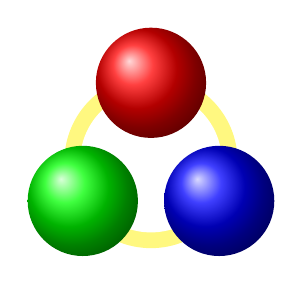
\begin{tikzpicture}
\path[fill=yellow!50!white] (0,0) circle (11mm);
\path[fill=white] (0,0) circle (9mm);
\foreach \w/\c in {90/red,210/green,330/blue}
{\path[shading=ball,ball color=\c] (\w:1cm) circle (7mm);}
\end{tikzpicture}
\end{texexptitled}
\end{dispExample}


\begin{dispExample}
\begin{texexptitled}[center lower,enhanced,segmentation hidden,middle=0mm]
{How to use options (2):\par The text output is centered and the
segmentation line has vanished.}{options2}
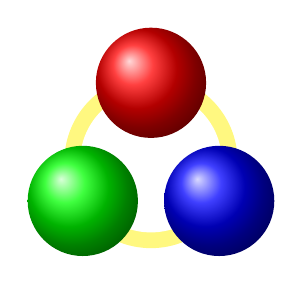
\begin{tikzpicture}
\path[fill=yellow!50!white] (0,0) circle (11mm);
\path[fill=white] (0,0) circle (9mm);
\foreach \w/\c in {90/red,210/green,330/blue}
{\path[shading=ball,ball color=\c] (\w:1cm) circle (7mm);}
\end{tikzpicture}
\end{texexptitled}
\end{dispExample}

\begin{dispExample}
\begin{texexptitled}[tikz lower,bicolor,colbacklower=white]
{How to use options (3):\par Here, the |tikzpicture| is totally hidden.
The |bicolor| skin highlights the output.}{options3}
\path[fill=yellow!50!white] (0,0) circle (11mm);
\path[fill=white] (0,0) circle (9mm);
\foreach \w/\c in {90/red,210/green,330/blue}
{\path[shading=ball,ball color=\c] (\w:1cm) circle (7mm);}
\end{texexptitled}
\end{dispExample}

\begin{dispExample}
\begin{texexptitled}[center lower,listing side text,righthand width=3.5cm,
bicolor,colbacklower=white]
{How to use options (4):\par The |bicolor| skin also works with side
by side mode}{options4}
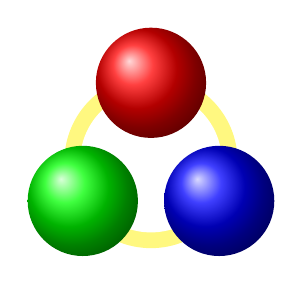
\begin{tikzpicture}
\path[fill=yellow!50!white] (0,0) circle (11mm);
\path[fill=white] (0,0) circle (9mm);
\foreach \w/\c in {90/red,210/green,330/blue}
{\path[shading=ball,ball color=\c]
(\w:1cm) circle (7mm);}
\end{tikzpicture}
\end{texexptitled}
\end{dispExample}


\begin{dispExample}
\begin{texexptitled}[center lower,listing outside text,righthand width=3.5cm]
{How to use options (5):\par Putting our picture outside is just
a matter of one word.}{options5}
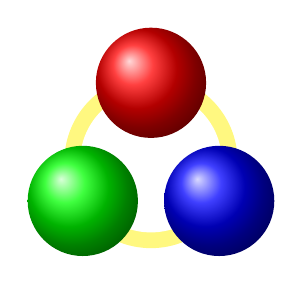
\begin{tikzpicture}
\path[fill=yellow!50!white] (0,0) circle (11mm);
\path[fill=white] (0,0) circle (9mm);
\foreach \w/\c in {90/red,210/green,330/blue}
{\path[shading=ball,ball color=\c]
(\w:1cm) circle (7mm);}
\end{tikzpicture}
\end{texexptitled}
\end{dispExample}


\begin{dispExample}
\begin{texexptitled}[center lower,text above listing]
{How to use options (6):\par The picture may also be put above
the listing box.}{options6}
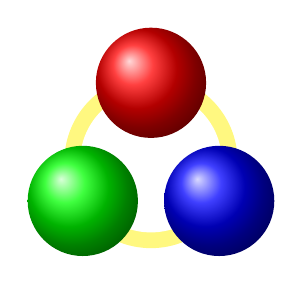
\begin{tikzpicture}
\path[fill=yellow!50!white] (0,0) circle (11mm);
\path[fill=white] (0,0) circle (9mm);
\foreach \w/\c in {90/red,210/green,330/blue}
{\path[shading=ball,ball color=\c]
(\w:1cm) circle (7mm);}
\end{tikzpicture}
\end{texexptitled}
\end{dispExample}


\begin{dispExample}
\begin{texexptitled}[beamer,center lower,text outside listing,lefthand width=3.5cm]
{How to use options (7):\par Our style is easily transformed into
a beamerish one.}{options7}
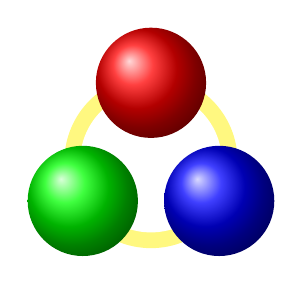
\begin{tikzpicture}
\path[fill=yellow!50!white] (0,0) circle (11mm);
\path[fill=white] (0,0) circle (9mm);
\foreach \w/\c in {90/red,210/green,330/blue}
{\path[shading=ball,ball color=\c]
(\w:1cm) circle (7mm);}
\end{tikzpicture}
\end{texexptitled}
\end{dispExample}

% % \clearpage
% \subsection{Creation of \LaTeX\ Exercises\\\LaTeX\ 练习的创建}\label{listing:exercises}
% \subsection{Creation of \LaTeX\ Exercises\\\LaTeX\ 练习的创建}\label{listing:exercises}

In the following, a guideline is given for the creation of \LaTeX\ exercises
with solutions. These solutions are saved to disk for application at a place of
choice.
Therefore, all used exercises are logged to a file |\jobname.records| for automatic
processing. The solution contents themselves are saved to a subdirectory named
|solutions|. Also see \Vref{sec:recording}.

下面提供了一个指南,用于创建带有答案的 \LaTeX\ 练习。这些答案被保存到磁盘上,以便在需要的地方应用。因此,所有使用的练习都被记录在一个名为 |\jobname.records| 的文件中\footnote{比如tcolorbox.records。}%
,以便自动处理。解答内容本身保存在一个名为 |solutions| 的子目录中。请参见 \Vref{sec:recording}。
\begin{itemize}
\item Before the first exercise is given,
\refComLe{tcbstartrecording} has to be called to start recording.
\\在给出第一个练习之前,必须调用 \refComLe{tcbstartrecording} 开始录制。
\item The solution is given as content of a \refEnvLe{tcboutputlisting}
environment. Note, that you can use this content also inside the
exercise with \refComLe{tcbuselistingtext} in compiled form.
\\解决方案作为 \refEnvLe{tcboutputlisting} 环境的内容给出。请注意,您可以使用编译后的形式在练习中使用 \refComLe{tcbuselistingtext}。
\item After the last exercise is given (and before using the solutions),
\refComLe{tcbstoprecording} has to be called to stop recording.
\\在给出最后一个练习(且在使用解决方案之前),必须调用 \refComLe{tcbstoprecording} 停止录制。
\item The solutions are loaded by \refComLe{tcbinputrecords}.
\\解决方案通过 \refComLe{tcbinputrecords} 加载。
\end{itemize}

Inside the exercise text, there may be text parts which are needed as
\LaTeX\ source code and as compiled text as well. These parts can be
saved by \refEnvLe{tcbwritetemp} and used in compiled form by \refComLe{tcbusetemp}
or as source code by \refComLe{tcbusetemplisting}.

在练习文本中,可能存在需要作为\LaTeX 源代码和编译后文本的文本部分。这些部分可以通过\refEnvLe{tcbwritetemp}保存,并通过\refComLe{tcbusetemp}以编译形式使用,或通过\refComLe{tcbusetemplisting}作为源代码使用。

At first, we generate some a common style for the exercises and the
solutions. Further, since exercises and solutions should
be numbered, we force to use a label \meta{marker}.
Automatically, the label |exe:|\meta{marker} is used to mark the exercise
and the label |sol:|\meta{marker} is used to mark the solution.

首先,我们为练习和解决方案生成了一种常见的样式。另外,由于练习和解决方案需要编号,我们强制使用标签\meta{marker}。自动地,标签|exe:|\meta{marker}用于标记练习,而标签|sol:|\meta{marker}用于标记解决方案。

\begin{dispListing}
\tcbset{texercisestyle/.style={arc=0.5mm, colframe=blue!25!yellow!90!white,
colback=blue!25!yellow!5!white, coltitle=blue!25!yellow!40!black,
fonttitle=\small\sffamily\bfseries, fontupper=\small, fontlower=\small,
listing options={style=tcblatex,texcsstyle=*\color{red!40!black}},
}}
\end{dispListing}
\tcbusetemp

With these preparations, the kernel environment |texercise| for our
exercises is created quickly:

有了这些准备,我们的练习内核环境 |texercise| 就能够快速创建:

\inputpreamblelisting{E}

%% \clearpage
The following examples demonstrate the application.

以下示例演示了应用程序。

\begin{dispListing}
\tcbstartrecording
\end{dispListing}
\tcbusetemp


\begin{dispExample}
\begin{texercise}{tabular_example}
\textit{Create the following table:}\par\smallskip%
\begin{tcboutputlisting}
\begin{tabular}{|p{3cm}|p{3cm}|p{3cm}|p{3cm}|}\hline
\multicolumn{4}{|c|}{\bfseries\itshape Das alte Italien}\\\hline
\multicolumn{2}{|c|}{\bfseries Antike} &
\multicolumn{2}{c|}{\bfseries Mittelalter}\\\hline
\multicolumn{1}{|c|}{\itshape Republik}&
\multicolumn{1}{c|}{\itshape Kaiserreich}&
\multicolumn{1}{c|}{\itshape Franken}&
\multicolumn{1}{c|}{\itshape Teilstaaten}\\\hline
In den Zeiten der r\"{o}mischen Republik standen dem Staat jeweils zwei
Konsuln vor, deren Machtbefugnisse identisch waren. &
Das r\"{o}mische Kaiserreich wurde von einem Alleinherrscher, dem Kaiser,
regiert.
& In der V\"{o}lkerwanderungszeit \"{u}bernahmen die Goten und sp\"{a}ter die
Franken die Vorherrschaft.
& Im sp\"{a}teren Mittelalter regierten F\"{u}rsten einen Fleckenteppich
von Einzelstaaten.\\\hline
\end{tabular}
\end{tcboutputlisting}
\tcbuselistingtext%
\end{texercise}
\end{dispExample}


\begin{dispExample}
\begin{texercise}{macro_oneparam}
\begin{tcboutputlisting}
\newcommand{\headingline}[1]{%
\begin{center}\Large\bfseries #1\end{center}}
\end{tcboutputlisting}
\tcbuselistingtext%

Create a new macro \verb+\headingline+ which produces the
following output:

创建一个新的宏\verb+\headingline+,它会产生以下输出:
\par\smallskip
\begin{tcbwritetemp}
\headingline{Very important heading}
\end{tcbwritetemp}
\tcbusetemplisting\tcbusetemp%
\end{texercise}
\end{dispExample}



\begin{dispExample}
\begin{texercise}{macro_twoparam}
\begin{tcboutputlisting}
\newcommand{\minitable}[2]{%
\begin{center}\begin{tabular}{p{10cm}}\hline%
\multicolumn{1}{c}{\bfseries#1}\\\hline%
#2\\\hline%
\end{tabular}\end{center}}
\end{tcboutputlisting}
\tcbuselistingtext%
Create a new macro \verb+\minitable+ which produces the
following output:

创建一个名为\verb+\minitable+的新宏,它会生成以下输出\par\smallskip
\begin{tcbwritetemp}
\minitable{My heading}{In this tiny tabular, there is only a heading
and some text below which has a width of ten centimeters.}
\end{tcbwritetemp}
\tcbusetemplisting\par\smallskip\tcbusetemp%
\end{texercise}
\end{dispExample}


\begin{dispExample}
\begin{texercise}{macro_threeparam}
\begin{tcboutputlisting}
\newcommand{\synop}[3]{%
\begin{tabular}{@{}p{(\linewidth-\tabcolsep*2-\arrayrulewidth)/2}|%
p{(\linewidth-\tabcolsep*2-\arrayrulewidth)/2}@{}}\hline
\multicolumn{2}{c}{\bfseries #1}\\\hline
\multicolumn{1}{c|}{\itshape English}&
\multicolumn{1}{c}{\itshape German}\\\hline
#2 & #3
\end{tabular}}
\end{tcboutputlisting}
\tcbuselistingtext%
Create a new macro \verb+\synop+ which typesets a synoptic text according
to the following example. Base your macro on a tabular which takes the
total line width.

创建一个新的宏\verb+\synop+,根据以下示例排版综合文本。基于一个接受总行宽的表格来创建你的宏。\par\smallskip
\begin{tcbwritetemp}
\synop{Neil Armstrong}%
{That's one small step for a man, one giant leap for mankind.}%
{Das ist ein kleiner Schritt f\"{u}r einen Mann,
ein riesiger Sprung f\"{u}r die Menschheit.}
\end{tcbwritetemp}
\tcbusetemplisting\par\smallskip\tcbusetemp%
\end{texercise}
\end{dispExample}
%\closeoutsol

\begin{dispListing}
\tcbstoprecording
\end{dispListing}
\tcbusetemp

\bigskip

Now, we give a list of all exercises with:

现在,我们列出了所有练习的清单,包括:
\begin{dispListing}
\tcblistof[\subsection]{exam}{List of Exercises%
\label{listofexercises}}
\end{dispListing}
\tcbusetemp

% %% \clearpage
% \subsection{Solutions for the given \LaTeX\ Exercises\\\LaTeX\ 练习的解决方案}

% For all solutions, a macro |\processsol| was written to the file |\jobname.records|.
% Now, we need a definition for this macro to use the solutions.

% 对于所有的解决方案,一个名为 |\processsol| 的宏已经被写入到文件 |\jobname.records| 中。 现在,我们需要一个定义来使用这个宏来处理解决方案。
% \begin{dispListing}
% % \usepackage{hyperref} % for phantomlabel
% \newtcbinputlisting{\processsol}[2]{%
%   texercisestyle,
%   listing only,
%   listing file={#1},
%   phantomlabel={sol:#2},%
%   title={Solution for Exercise \ref{exe:#2} on page \pageref{exe:#2}},
% }
% \end{dispListing}
% \tcbusetemp

% The loading of all solutions is done by:

% 所有解决方案的加载是通过以下方式完成的:

% \begin{dispListing}
% \tcbinputrecords
% \end{dispListing}

% With this, we get:

% 通过这个,我们得到:

% \tcbusetemp



